\documentclass[10pt]{article}
\usepackage[utf8]{inputenc}
\usepackage{url}
\usepackage{graphicx}
\usepackage[table]{xcolor}
\usepackage{blindtext}
\usepackage{enumitem}
\usepackage{booktabs}

\title{First document}
\author{Group 3}
\date{October 2018}

\begin{document}
\section{Avi System Software Design and Architecture Document} \\

\textbf{Version 1.3} \\

\begin{center}
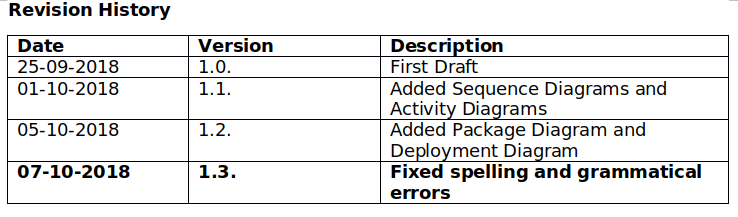
\includegraphics[width=.9\textwidth]{revision_history.png}
\end{center}
\caption{\underline{Revision History}}

\subsection{Introduction}

This section provides an overview of this document. It includes the purpose, scope, definitions and acronyms, references and overview of the system.

\subsubsection{Purpose}

The main purpose of this document is to provide the design and architectural overview of the Avi System. It presents the architectural decisions made in designing and developing the system. This document can be used by the project stakeholders (developers and client) to better understand the problem being solved and how the Avi System will represent the solution.

\subsubsection{Scope}

Avi is a web application that will recommend elective courses to prospective postgraduate students and further predict the grades the students are likely to get in the recommended courses based on their grades in previously completed courses.

A student will start by creating an account which includes specifying their first name, surname, student number, highest completed level of study and their login password.

Once a student has created an account they can only be able to get recommendations once they have added the courses they have done and the grade they obtained in the courses. This information can be updated by the student for cases where they may have made a mistake or their mark has changed.

The student can now request to get recommendations. After this the system will present to them the recommended courses along with the predicted grade for each course.

\subsubsection{Definitions, Acronyms and Abbreviations}
PC:  Personal computer
Client: University of Witwatersrand
** See the Glossary Document for system definitions **
\subsubsection{References}
** COME BACK **

\subsubsection{Overview}

The next section, section 2, of this document describes the goals and constraints of designing the system’s architecture. Section 3 describes the architectural representation of the system. Section 4 describes the 5 different ways in which the system architecture can be viewed.  describes all the software requirements. Section 5 describes the system’s size and performance and Section 6 talks about the system’s quality concerns.

\subsection{Architectural Goals and Constraints}

The architecture design of the Avi System was influenced by the requirements specified in the System Requirements Specification document and it was constrained by the Django framework architecture.

\subsection{Architectural Representation}


\subsubsection{Architectural Design Pattern and Architectural Style}

The Avi System follows the Model-Template-View (MTV) design pattern. The model is the data access layer, it is a representation of the database and contains everything about how to access the data.  The template is the presentation layer, it is what the user sees and interacts with. The view is the business logic layer, it controls the flow of information between the models and templates and is responsible for any processing.

\begin{center}
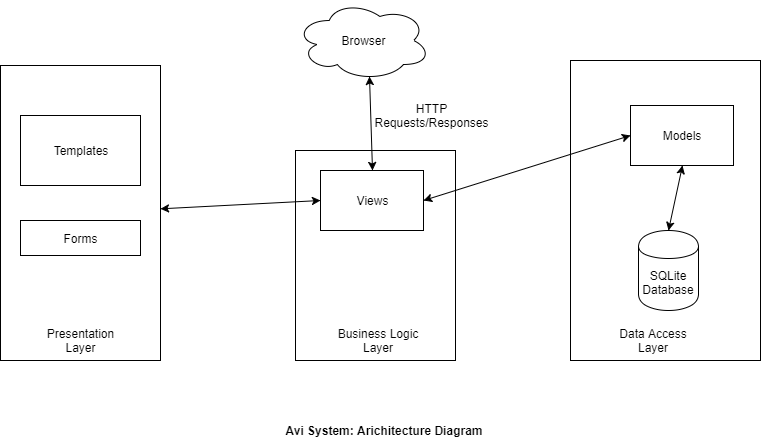
\includegraphics[width=.9\textwidth]{architecture_diagram.png}
\end{center}
\caption{\underline{Architecture Diagram}}

\newpage

\subsubsection{Architectural Views}
This section describes the system from different perspectives of the project stakeholders. The image below illustrates the views considered.
\begin{center}
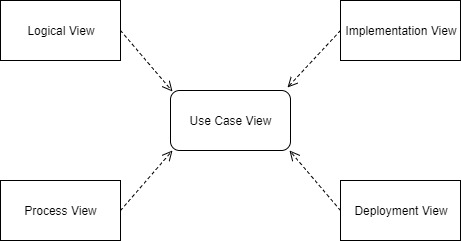
\includegraphics[width=.9\textwidth]{architecture_views.png}
\end{center}
\caption{\underline{Architectural Views}}

\section{Architectural View Decomposition}

\subsection{Use Case View}

The use case view depicts the system from the users’ perspective. In this section we have focused on three use cases which we believe are crucial to the running of the system, these use cases are Create Account, Add Course and Get Recommendation.

\subsubsection{Use Case Diagram}
This Use Case Diagram is a subset of the final Use Case Diagram found in the System Requirements Specification document.
\begin{center}
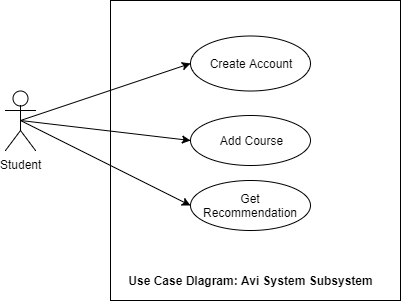
\includegraphics[width=.9\textwidth]{use_case_diagram.png}
\end{center}
\caption{\underline{Use Case Diagram}}

\subsubsection{Use Case Descriptions}

\paragraph{1. Create Account \\}

Main Success Scenario: \\
The use case starts when the user requests to create an account. The system will prompt the user to enter their details (i.e. their first name, surname, student number, highest completed level of study and their login password). The user will enter these details and commit the details by pressing the ‘Create Account’ button. The system will check that the password and confirmation of password match. If they match, the system will create the account and the user will be redirected to the login page.

Alternative Scenario: \\
S1: If the password and confirmation of password do not match the use case will be restarted.

\paragraph{2. Add Course \\}

Main Success Scenario: \\
The use case starts when the user requests to add a course. The system will prompt for a course code and the grade obtained in the course. The user will enter these details and  commit the details by pressing the ‘Add Course’ button. The system will validate (i.e. Check if the course code exists and if the entered grade is a number between 0 and 100) the details and if they are valid it will then add the course and the added course will appear under the ‘Your Courses’ section of the page.

Alternative Scenario: \\
S1: If the details are invalid the use case will be restarted.

\paragraph{3. Get Recommendation \\}

Main Success Scenario:\\
The use case is started when the user requests to get a recommendations. The system will check if the user has added courses to their profile. If they have, the system will generate the recommendations and they will appear under the ‘Your Recommendations’ section of the page.

Alternative Scenario:\\
S1: If the user does not have any courses added to their profile, the use case will halt and the user will be advised by the system to add their courses before requesting a recommendation.

\subsection{Logical View}

This view is concerned with depicting the functionality provided to the users by the system. This is done using class and state diagrams.
\begin{center}
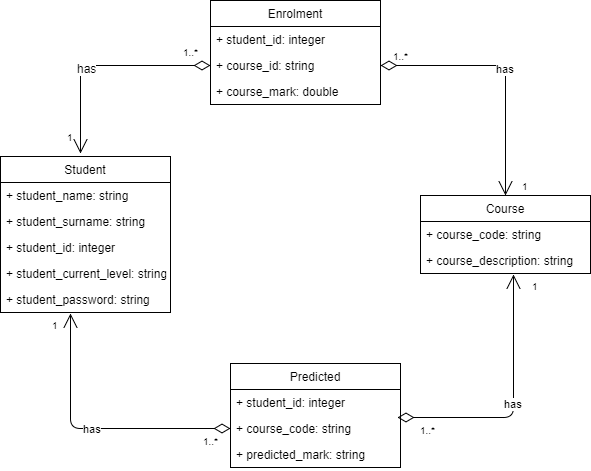
\includegraphics[width=.9\textwidth]{class_diagram.png}
\end{center}
\caption{\underline{Class Diagram}} \\ \\

\textbf{Note:} The AVI System does not contain any state changes. Thus there is no state diagram. 

\subsection{Process View}

This view demonstrates the processes that form part of the system and how they interact with each other. It focuses largely on concurrency and the sequence of processes.


\paragraph{Activity Diagrams \\}
These diagrams are a graphical representation of multiple business processes, specifically, the Create Account, Add Course and Get Recommendation business processes. They show the data flow and the control flow of the business processes.

\begin{center}
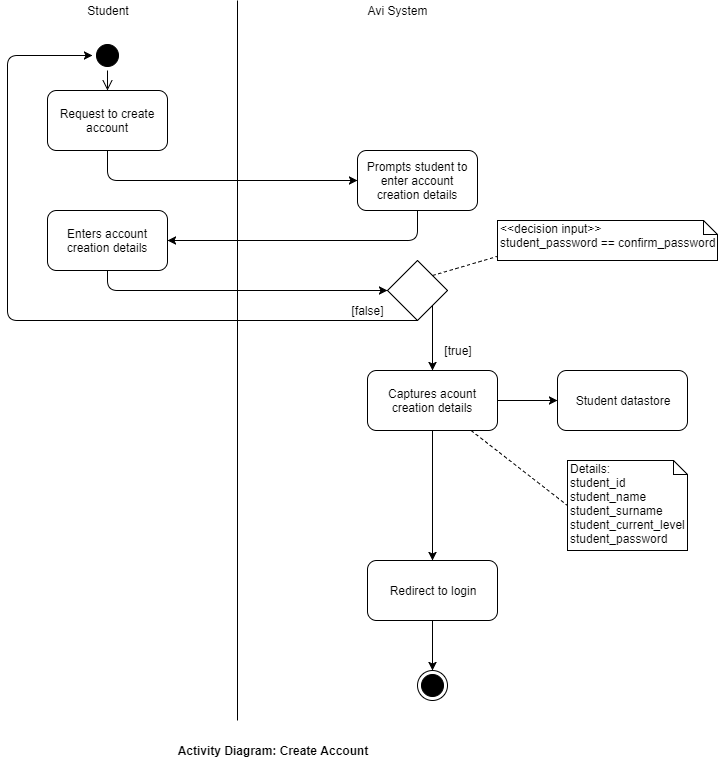
\includegraphics[width=.9\textwidth]{activity_diagram_create_account.png}
\end{center}
\caption{\underline{Activity Diagram: Create Account}}

\newpage

\begin{center}
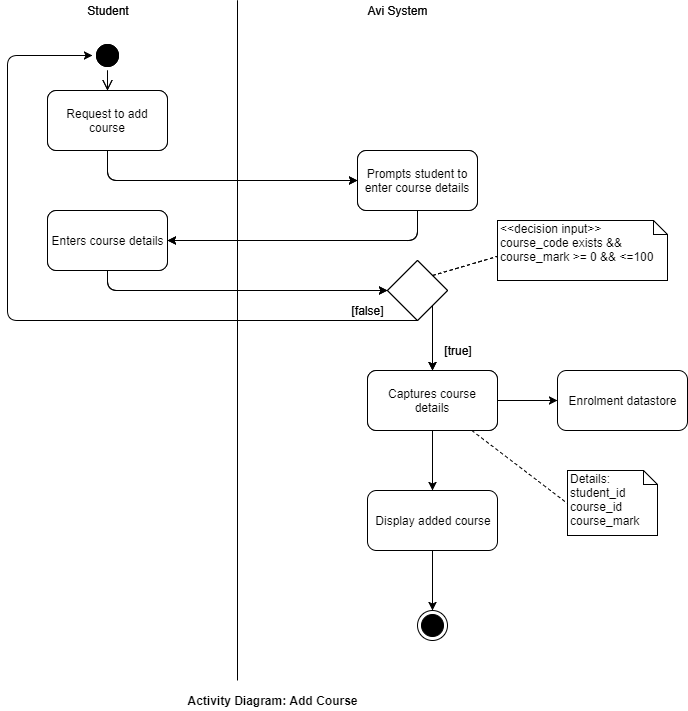
\includegraphics[width=.9\textwidth]{activity_diagram_add.png}
\end{center}
\caption{\underline{Activity Diagram: Add Course}} \\ \\

\begin{center}
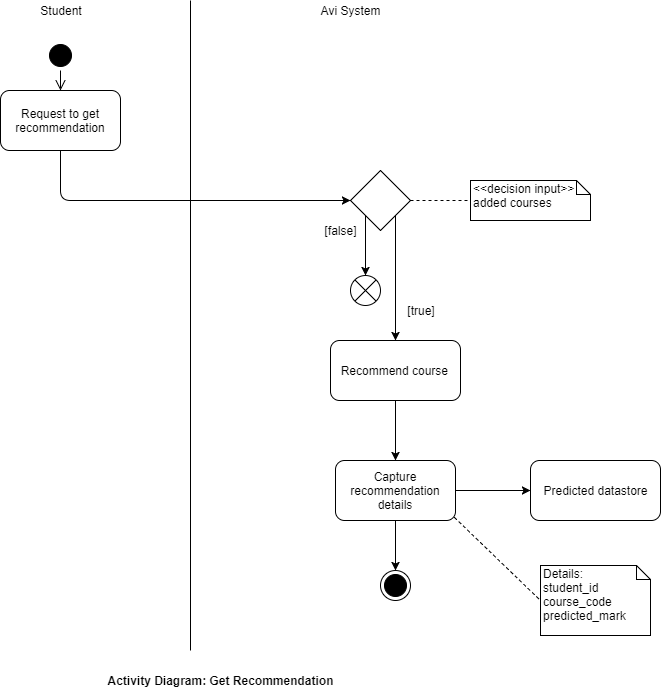
\includegraphics[width=.9\textwidth]{activity_diagram_get.png}
\end{center}
\caption{\underline{Activity Diagram: Get Recommendation}}

\paragraph{Sequence Diagrams \\}

The purpose of these diagrams is to illustrate the communication between the actor and system during the Create Account, Add Course and Get Recommendations processes.

\begin{center}
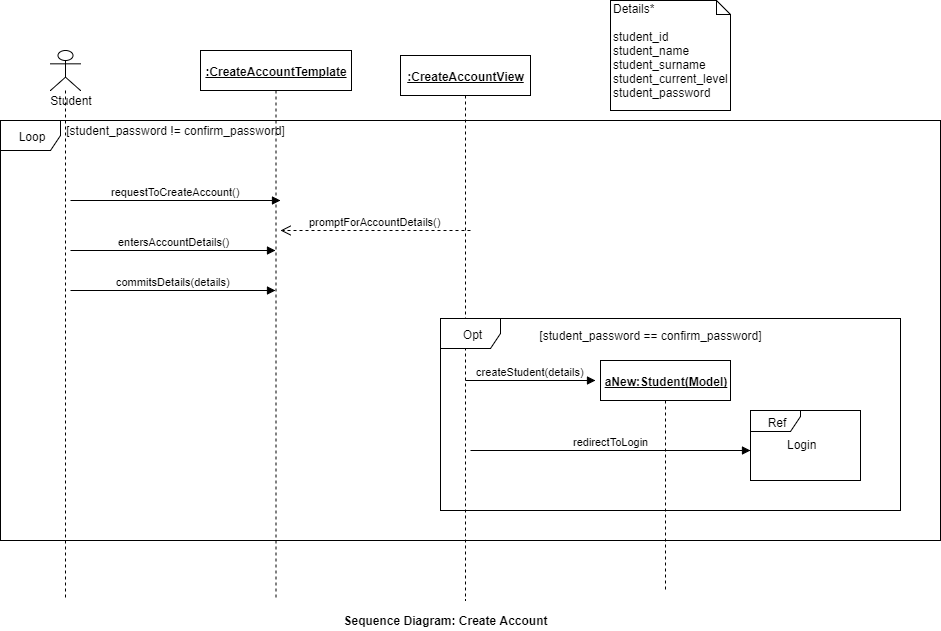
\includegraphics[width=.9\textwidth]{sequence_diagram_create.png}
\end{center}
\caption{\underline{Sequence Diagram: Create Account}}



\begin{center}
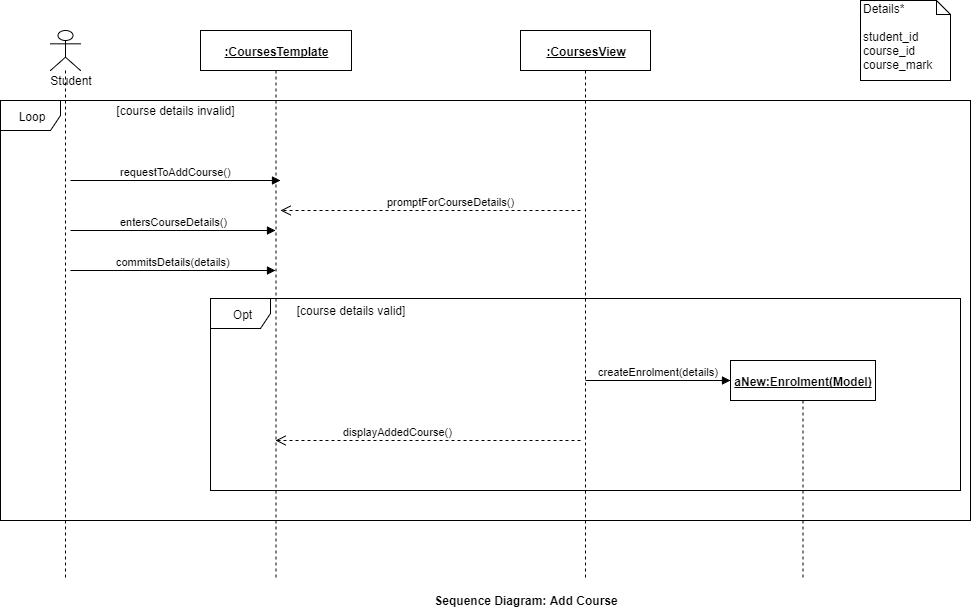
\includegraphics[width=.9\textwidth]{sequence_diagram_add.png}
\end{center}
\caption{\underline{Sequence Diagram: Add Course}} \\ \\

\begin{center}
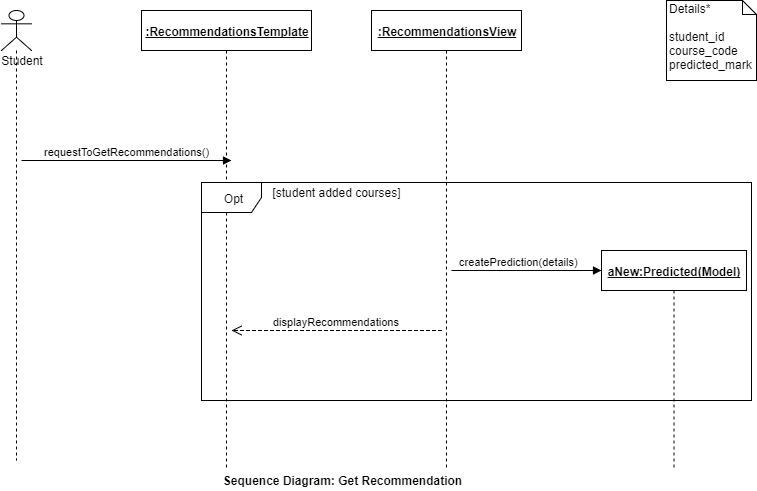
\includegraphics[width=.9\textwidth]{sequence_diagram_get.png}
\end{center}
\caption{\underline{Sequence Diagram: Get Recommendation}} \\ \\

\subsection{Implementation View}

This view depicts the system from the developer’s perspective. It describes the system’s modules in terms of packaging, layering and configuration.

\begin{center}
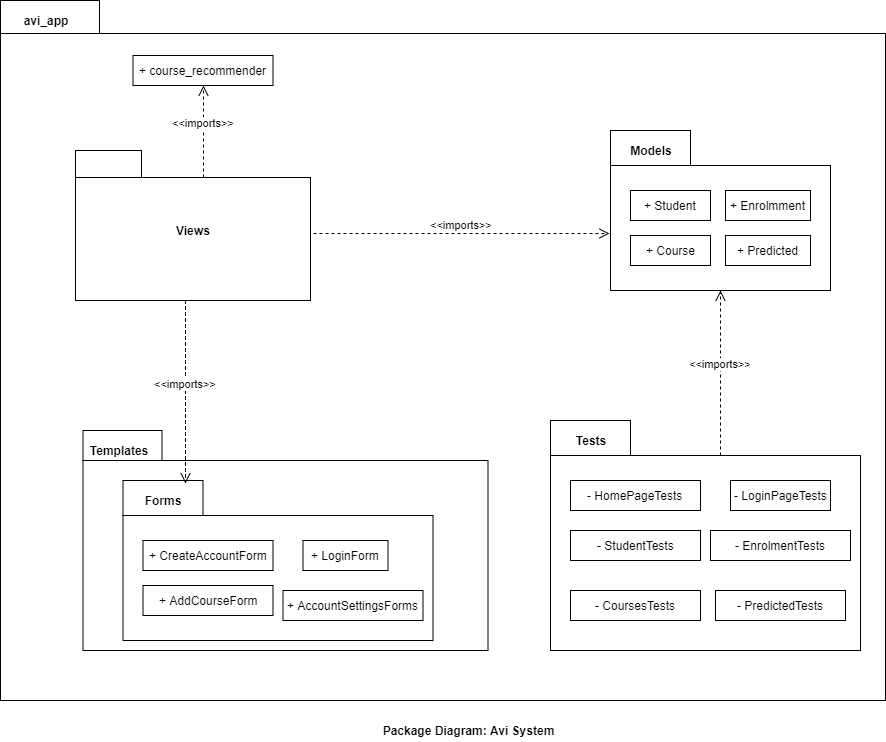
\includegraphics[width=.9\textwidth]{package_diagram.png}
\end{center}
\caption{\underline{Package Diagram: Avi System}} \\ \\

\subsection{Deployment View}

This view depicts the system from the engineer’s point of view. It depicts the physical components on which the system runs on. The diagram below only depicts the system’s deployment diagram in the development environment since we do not move it to a production environment

\begin{center}
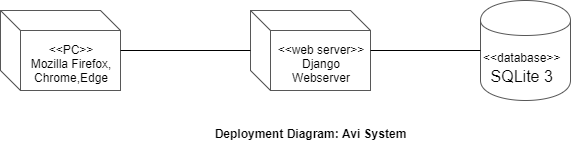
\includegraphics[width=.9\textwidth]{deployment_view.png}
\end{center}
\caption{\underline{Deployment Diagram: Avi System}}

\subsection{Size and Performance}

Below is a summary of the system’s size and performance.

\begin{description}[font=$\bullet$~\normalfont\scshape\color{red!50!black}]
\item[] The size of the system (classes, packages etc.) is approximately 2.2 MB.
\item[] The size above does not include the external libraries and software that need to be installed.
\end{description}


\subsection{Quality}

This system is not entirely reliable mainly because this was a prototype to demonstrate how the final system would operate. 

\begin{description}[font=$\bullet$~\normalfont\scshape\color{red!50!black}]
\item[] Password encryption was not implemented.
\item[] It depends on the operating system and database security features.
\item[] Difference user’s data is protected i.e. No user has access to another user’s data.
\end{description}


\end{document}

